\chapter{Architecture}
    \section{High Level Overview}
        The system is composed of 2 main components
        \begin{itemize}
            \item wslmon - an sdk that contains the detection logic as well as communication logic between kernel-mode and user-mode
            \item wslam - the integrator
        \end{itemize}

        Below we can see a high level overview of the sdk and integrator components and how they can interract.
        
        \begin{figure}[H]
            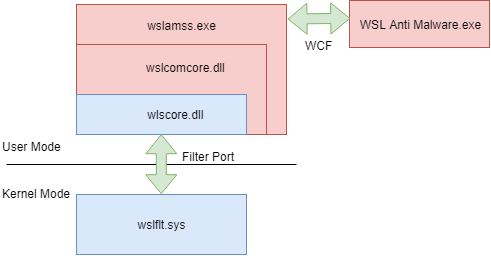
\includegraphics[width=360px, keepaspectratio]{img/high_level_overview_diagram.png}
            \caption{High Level Overview}
            \label{fig:high_level_overview_diagram}
        \end{figure}

        Blue colored components are part of the wslmon SDK, while the red colored components are the integrator components.
    
    \subsection{wslmon}
        Wslmon is an SDK that could be integrated by any OEM to include it in an existing security solution. Its
        architecture is meant to provide an easy way of integration in real anti-virus products, offer enough control of the system while
        encapsulating the monitoring and detection logic algorithms.

        The SDK consists of two components:
        \begin{itemize}
            \item wslflt.sys - a minifilter driver that encapsulates the monitoring, analysis and detection logic
            \item wslcore.dll - a shared library that provides an interface to communicate with the minifilter driver
        \end{itemize}

        \paragraph{wslflt.sys}
        is a C++ minifilter driver that contains the requirued sensors for monitoring process' activity. It's key components are the
        process filter, file filter, event dispatcher, the communication framework and the detection heuristics.

        \paragraph{wslcore.dll}
        is meant to ease the integration process of the sdk by third party anti-virus vendors. It offers an interface for controlling the driver
        state (enable/disable monitoring) as well as callback registration for several events (i.e detection).

    \subsection{wslam}
        Integrating the wslmon SDK, it consists of:
        
        \begin{itemize}
            \item wslcomcore.dll - C++/CLI DLL
            \item wslamss.exe - .NET Service
            \item WSL Anti-Malware.exe - WPF GUI Application
        \end{itemize}

        \paragraph{wslcomcore.dll} is built on top of C++/CLI to wrap wslcore.dll and export managed .NET classes
        for use in the .NET service. It's main purpose is to hide the filtering and detection logic and to provide an easy way to integrate
        the system in a complete security solution.

        \paragraph{wslamss.exe} contains the integration logic (ie. detection notifications, logging, etc) and serves as a communication
        endpoint, built using WCF framework, for the GUI application. It uses the previously mentioned dll to control the driver state, process
        driver's notifications as well as reqests sent from the GUI application. It is designed as a Windows Service application, therefore,
        making it easily convertible to an anti-malware protected process, once an Early Launch Anti-Malware (ELAM) driver is properly signed.

        \paragraph{WSL Anti-Malware.exe}
        is the GUI application that gives control to the user while also containing the user notification mechanism. It is designed as a system
        tray application in order to not distrupt the user experience, while the GUI itself is designed for usability.

    \section{SDK Architecture}
        The driver, which is responsilbe with monitoring of processes and detection of potentially malicious applicatoins, is comprised of
        two "sensors", the first being responsible of monitoring process creation and termination, called ProcessFilter, and the second being
        responsible of filtering file system I/O operations, called FileFilter.

        Most of the main components in the driver are implemented as singleton classes, and that is because of the inherent architecture of
        the minifilter APIs. For example, the callback for process notification has no context parameter, making it impossible to access
        any other component, except through singleton classes.

        \subsection{Process Filter}
        The process filter is a stateful component, in the snese that the filter can be enabled or disabled, and responsible for registering
        the callback for process creation and termination notifications. It contains the logic for deciding whether or not a process should be
        monitored.

        It also contains a process collector, which is used as a databse of active processes, internally represented by instaces of the Process
        class. A Process object holds the needed information for uniquely identifying the process throughout it's lifetime as well as other
        information useful for behavioral analysis, like the parent process, security token or commandline.

        \subsection{File Filter}
        The file filter is also a stateful and singleton component. It's responsible for providing the IRP filtering callbacks and analyzing
        potentially malicious file system activity.

        Currently, the following operations are being monitored by the file filter:

        \begin{itemize}
            \item IRP\textunderscore MJ\textunderscore CREATE
            \item IRP\textunderscore MJ\textunderscore WRITE
        \end{itemize}
        
    \section{Integration Architecture}
    The SDK integration logic is encapsulated into a wslamss .NET Windows service application and is the juncture between the SDK and any 
    client application which would serve as a user interface.

    This architecture makes the integration project highly extensible, allowing the developement of a central application that can monitor
    reported incidents and other events from multiple clients (systems with the anti-malware solution installed). For example, this could be
    useful for the network administrators or security reposibles in business enviroments, allowing for faster incident response.
    
    \paragraph{}
    The service has an external-facing WCF interface which is accessible trhough the net.tcp://localhost:8000. The metadata is available at
    net.tcp://localhost:8000/mex. The metadata exchange endpoint is done via SOAP messages that contain various information that describes
    the service, such as: available operations, parameter types, return types, callbacks that need to be implemented, etc. In other words,
    the metadata exchange endpoint exposes the WCF contract implemented by the service.

    


        